\chapter{Asking A Billionaire Lawyer How To Make \$1{,}000{,}000!}

This School of Hard Knocks interview, curated here for the LazyEarn track by LazyingArt LLC, is not a blackboard lecture in the usual sense. Its mathematics lies in business arithmetic: how a personal-injury firm aligns incentives, converts reach into cases, converts cases into recoveries and fees, and then protects the resulting capital from ruin. Since no validated mathematical frames survive for this lecture, the equations and diagrams below are cautious transcript-derived reconstructions rather than transcriptions from a visible board. The tape itself opens twice, first as spectacle and then as explanation, and we will keep that rhythm. The question is not merely how rich John Morgan became; it is how a law practice was turned into a scalable machine.

\section{Opening Field: A Rare Billionaire Route}

The lecture begins with a teaser montage that flashes the themes before they are explained: billionaire status, a very large year, business conflict, humble origins, entrepreneurial selection, and a final life-principle question. Only after this quick burst does the host reset and give the real frame. Morgan is interesting not just because he is rich, but because the route to that wealth runs through law, which the host treats as rare enough to count on fewer than two hands.

That opening matters. We are not yet being asked to admire a mansion; we are being asked to notice an unusual commercial path. The host insists that billionaire-scale wealth built through legal practice is uncommon, and then drives to Morgan's house with that rarity in mind. The narrative motion is from spectacle to mechanism.

Once the interview settles at the front of the house, Morgan identifies the core business plainly: personal injury law. He then adds the scale claim that controls the rest of the chapter: he built what he calls the largest PI law firm in North America. The early question about money is therefore not merely gossip; it is a way of fixing the size of the object before we ask how it works.

In its later and more precise form, the annual scale is stated as
\begin{equation}
F \approx \$2 \times 10^9,
\end{equation}
where \(F\) denotes annual fees. That number is not yet an explanation. It is a marker placed on the table so that the explanatory question can become sharp: what single operating decision allowed a law firm to grow to this scale?

\section{Delegation, Profit-Sharing, and the First Scale Law}

Morgan's first answer is remarkably direct: delegate, find partners one can trust, and share the business with them. The lecture wants to get past biography and into mechanism quickly, and this is the first mechanism. The founder does not scale by doing more of everything himself; he scales by building a structure in which able people participate in the upside.

A compact way to record the economic idea is
\begin{equation}
\Pi_{\mathrm{firm}} = \Pi_{\mathrm{founder}} + \sum_{i=1}^{n}\Pi_i,
\end{equation}
where \(\Pi_{\mathrm{firm}}\) denotes total firm profit, \(\Pi_{\mathrm{founder}}\) the founder's share, and the \(\Pi_i\) the participating upside of trusted partners. This is not an accounting identity taken from the firm's internal books. It is a schematic representation of Morgan's phrase that good people must make money \emph{with} the founder, not merely \emph{for} him.

\begin{definition}
A \emph{send-delete} person is someone to whom a founder can send a task once, trust the execution, and then remove the task from active attention. In the lecture's shorthand we may record the operational rule as
\begin{equation}
\text{send} \to \text{trust} \to \text{delete}.
\end{equation}
\end{definition}

This is more than a hiring preference. It is a criterion for reducing managerial drag. A business in which the founder repeatedly reopens every delegated task has not really delegated anything. A business populated by send-delete people begins to acquire the resource that scale always consumes first: attention.

\begin{figure}
\centering
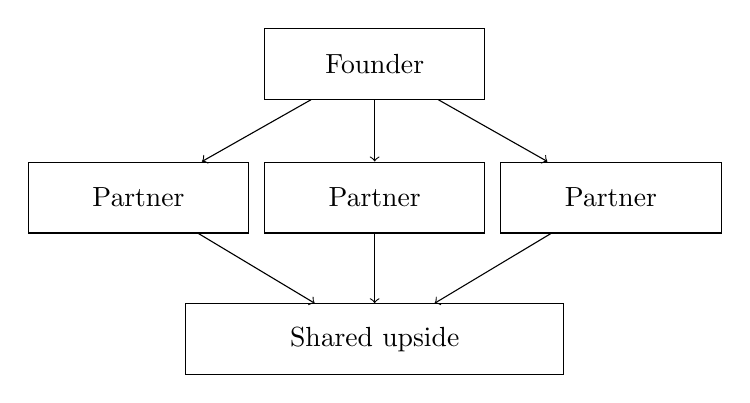
\begin{tikzpicture}[x=1cm,y=1cm]
\node[draw, rectangle, minimum width=2.8cm, minimum height=0.9cm] (f) at (0,2.2) {Founder};
\node[draw, rectangle, minimum width=2.8cm, minimum height=0.9cm] (p1) at (-3,0.5) {Partner};
\node[draw, rectangle, minimum width=2.8cm, minimum height=0.9cm] (p2) at (0,0.5) {Partner};
\node[draw, rectangle, minimum width=2.8cm, minimum height=0.9cm] (p3) at (3,0.5) {Partner};
\node[draw, rectangle, minimum width=4.8cm, minimum height=0.9cm] (s) at (0,-1.3) {Shared upside};
\draw[->] (f) -- (p1);
\draw[->] (f) -- (p2);
\draw[->] (f) -- (p3);
\draw[->] (p1) -- (s);
\draw[->] (p2) -- (s);
\draw[->] (p3) -- (s);
\end{tikzpicture}
\caption{Transcript-derived schematic of the first scale law: delegation plus shared profit.}
\label{fig:delegation-scale}
\end{figure}

The lecture then narrows one step further. Once we know that scale comes through people, the next question becomes what kind of people. Morgan's answer is not a personality test but an operating test: can the task leave the founder's attention without falling apart? That is the bridge from firm structure to personal biography.

\section{Pain, Purpose, and Who Is Built for the Game}

From delegation the lecture moves into motive. Morgan says he did not always know he would become a lawyer, but that his brother Tim was paralyzed in an accident while Morgan was in college. He describes anger at the way Tim was treated, and says that the event changed both of their lives. The later work of the firm is then narrated through that wound: when Morgan sees an injured client, he says he sees Tim.

This beat matters because it prevents the chapter from becoming a bloodless management memo. The commercial machine is not introduced as a neutral optimization device. It is introduced as a structure built by a person whose vocation was sharpened by grievance, loyalty, and a wish to protect people who resemble his brother.

The interview then broadens again. The host asks whether Morgan came from money, and Morgan answers with the memorable line that his father needed a cosigner to pay cash. That answer does two things at once. It denies inherited ease, and it clears the way for the next question: if the origin was not wealth, what was the turning point?

Morgan's answer is not a single event of financial discovery. He says instead that one is born with it. The paperboy becomes his emblem of entrepreneurial disposition: daily repetition, no vacation, and the early acquisition of commercial stamina. The later lion-and-sloth image is harsher, but it serves the same function. Not everybody, he says, is built for entrepreneurship.

We should be careful here. The lecture is not claiming that circumstances do not matter. It is claiming that a certain repetitive appetite for work often appears early. In the interview's order, this is important: first pain gives direction, then disposition determines whether one can bear the workload required to turn direction into scale.

\section{Contingency Fees, Negotiation, and the Contingent Path}

The host next asks what advice Morgan would give to a law student who wants to build an empire. The answer is immediate and structural. Morgan contrasts ordinary hourly billing with the contingency-fee model of personal injury practice. His complaint about hourly law is not that it is improper; it is that it offers too little upside for the type of game he wants to play.

A cautious reconstruction of the contrast is
\begin{equation}
F_{\mathrm{hourly}} = r h,
\end{equation}
where \(r\) is an hourly billing rate and \(h\) is billable time, while contingency practice is modeled by
\begin{equation}
F_{\mathrm{cont}} =
\begin{cases}
\alpha R, & \text{if the case is won},\\[4pt]
0, & \text{if the case is lost},
\end{cases}
\end{equation}
where \(R\) is the client's recovery and \(\alpha\) is the contingency fraction. These equations are editorial reconstructions of his verbal claim that he does not charge a fee unless he wins.

\begin{figure}
\centering
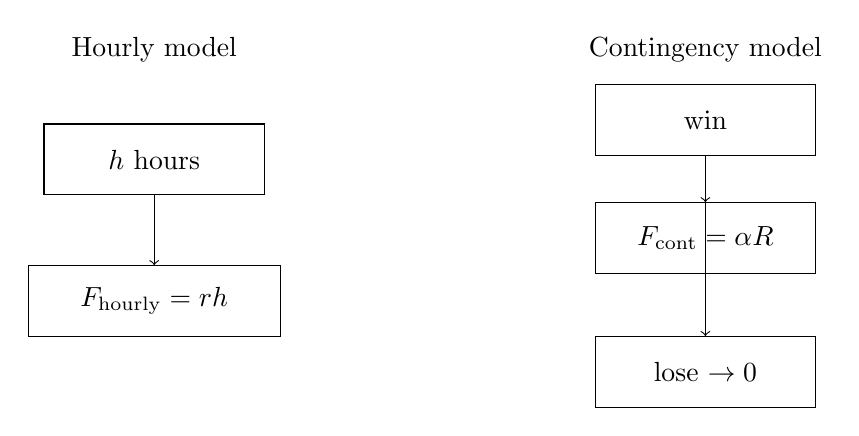
\begin{tikzpicture}[x=1cm,y=1cm]
\node at (-3.5,2.2) {Hourly model};
\node[draw, rectangle, minimum width=2.8cm, minimum height=0.9cm] (h1) at (-3.5,0.8) {\(h\) hours};
\node[draw, rectangle, minimum width=3.2cm, minimum height=0.9cm] (h2) at (-3.5,-1.0) {\(F_{\mathrm{hourly}} = rh\)};
\draw[->] (h1) -- (h2);

\node at (3.5,2.2) {Contingency model};
\node[draw, rectangle, minimum width=2.8cm, minimum height=0.9cm] (c1) at (3.5,1.3) {win};
\node[draw, rectangle, minimum width=2.8cm, minimum height=0.9cm] (c2) at (3.5,-0.2) {\(F_{\mathrm{cont}} = \alpha R\)};
\node[draw, rectangle, minimum width=2.8cm, minimum height=0.9cm] (c3) at (3.5,-1.9) {lose \(\to 0\)};
\draw[->] (c1) -- (c2);
\draw[->] (c1) -- (c3);
\end{tikzpicture}
\caption{Transcript-derived comparison of hourly billing and contingency participation in outcomes.}
\label{fig:fee-contrast}
\end{figure}

\subsection{Question \& Answer}

\paragraph{Question.} Why does Morgan think hourly billing is the wrong game if one wants empire-scale upside?

\paragraph{Answer.} Because hourly billing grows linearly with labor time, whereas contingency practice ties compensation to the magnitude of successful outcomes. Once a case is won, the schematic comparison becomes
\begin{equation}
\frac{F_{\mathrm{cont}}}{F_{\mathrm{hourly}}}
=
\frac{\alpha R}{r h}.
\end{equation}
Morgan's point is not that every contingency matter dominates every hourly matter. It is that if the firm is genuinely good at winning large recoveries, then the business model participates in outcomes rather than merely in elapsed time.

The lecture then pivots, almost casually, into negotiation. Morgan's aphorism is that whoever speaks first loses. We should not read this as mystical silence. The real point is informational. If we speak too early, we replace information with performance. Morgan says one must listen, learn, size up the deal, size up the person, and only then negotiate.

From there the lecture widens again into a philosophy of luck. Morgan says he has been hustling since childhood, but he also says life is luck: a thousand left turns, right turns, and U-turns, any one of which could have changed the outcome. The mathematical content here is modest but real. The interview is thinking in terms of path dependence rather than perfect self-authorship:
\begin{equation}
\omega = (d_1,d_2,\dots,d_n), \qquad d_k \in \{\text{left},\text{right},\text{U-turn}\},
\end{equation}
and the lecture's claim is that
\begin{equation}
d_k \mapsto d_k' \quad \Longrightarrow \quad O(\omega') \neq O(\omega),
\end{equation}
where \(O(\omega)\) denotes the terminal outcome generated by the path \(\omega\). This is not a theorem from probability theory. It is a disciplined way of preserving Morgan's insistence that successful people should be less self-congratulatory and more humble about contingency.

Mark Cuban is briefly invoked as corroboration, and faith enters in the same breath. Morgan says he believes in God and prays every night. The lecture then lands on what he calls the best advice from a mentor: keep your word. At this point the progression is clear. Fee structure determines the game, negotiation governs conduct inside the game, luck reminds us that the path is contingent, and reputation becomes one of the few durable assets that remains under deliberate control.

\section{Cutting Cancers and Managing the Human Side of the Machine}

The next movement is darker. The host asks whether Morgan has been wronged in business, and Morgan answers that he has, but that he responds. The lecture then becomes managerial rather than combative. Borrowing a line attributed to Jeff Bezos, Morgan says that sometimes one must pay people to walk away.

The metaphor he chooses is surgical. Bad actors are cancers in the business, and cancers must be excised. The lecture is explicit that negative energy is not merely unpleasant but commercially destructive. A poisonous internal node can absorb managerial attention far out of proportion to the revenue it touches. Hence the operating law is subtraction before escalation.

Another line in this sequence deserves to survive in the notes: the greatest revenge is success. That sentence does important work. It moves the interview away from vendetta and back toward construction. Even in conflict, the machine is healthiest when it is not organized around resentment.

The same tone appears when Morgan describes legal mistakes inside his own firm. Lawyers err; cases can be damaged. His answer is not concealment but admission. He says he brings the client in, says plainly that the lawyer made a mistake, and then points to insurance and the firm's balance sheet as the means of repair. In transcript-derived shorthand, the sequence is
\begin{equation}
\text{mistake} \to \text{disclosure} \to \text{insurance} \to \text{repair}.
\end{equation}
This is not a formal malpractice workflow. It is a compressed representation of the lecture's operating ethic: do not hide the error, and do not leave the client stranded with it.

At this point the video contains the host's promotional interlude about proximity, mentorship, and paid access. For our purposes, it should be acknowledged but heavily compressed. The chapter's rhythm is preserved if we note simply that the tape pauses, sells community, and then returns to the interview. When it returns, the lecture takes up its strongest strategic image.

\section{Competition, the Google Law Firm, and Brick-by-Brick Expansion}

The resumed interview begins with competition. Morgan welcomes it. Competition, he says, is what makes people great, and he uses Michael Jordan as the emblem of a person sharpened by rivalry rather than frightened by it. This is the motivational ramp into the major strategic thought experiment: what would Google do if it were a law firm?

That question functions almost like a theorem statement. Once it appears, the lecture reorganizes itself around availability. Morgan's answer is that such a firm would be everywhere for everyone: all \(50\) states, \(24/7\), and a client could become a client in about two minutes through a phone. A concise transcript-derived formalization is
\begin{equation}
\mathcal{C} = N_{\mathrm{states}} \times H_{\mathrm{service}} \times \tau_{\mathrm{intake}}^{-1},
\end{equation}
with
\begin{equation}
N_{\mathrm{states}} = 50, \qquad H_{\mathrm{service}} = 24/7, \qquad \tau_{\mathrm{intake}} \approx 2 \text{ min}.
\end{equation}
The notation is ours, not Morgan's. It simply preserves the logic that coverage rises with geography and uptime, and with the removal of intake friction.

\begin{figure}
\centering
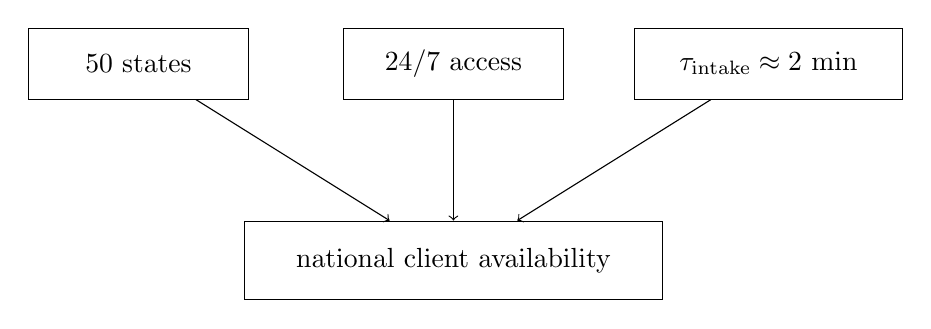
\begin{tikzpicture}[x=1cm,y=1cm]
\node[draw, rectangle, minimum width=2.8cm, minimum height=0.9cm] (a) at (-4,1.5) {\(50\) states};
\node[draw, rectangle, minimum width=2.8cm, minimum height=0.9cm] (b) at (0,1.5) {\(24/7\) access};
\node[draw, rectangle, minimum width=3.4cm, minimum height=0.9cm] (c) at (4,1.5) {\(\tau_{\mathrm{intake}} \approx 2\) min};
\node[draw, rectangle, minimum width=5.3cm, minimum height=1cm] (d) at (0,-1) {national client availability};
\draw[->] (a) -- (d);
\draw[->] (b) -- (d);
\draw[->] (c) -- (d);
\end{tikzpicture}
\caption{Transcript-derived schematic of the ``Google law firm'' idea: ubiquity, continuous access, and low-friction intake.}
\label{fig:google-law-refined}
\end{figure}

The host then supplies a useful bit of evidence from outside the theory: when he told people he was interviewing John Morgan, they already knew the brand. In other words, the Google-law-firm vision is not left as aspiration; it is presented as something the public already partially recognizes.

\subsection{Question \& Answer}

\paragraph{Question.} What does it actually mean to scale a service business nationally without collapsing quality?

\paragraph{Answer.} In the lecture it means two things at once. First, reduce access friction: broad geography, continual availability, rapid intake. Second, refuse to confuse access with execution. Morgan will later insist that marketing without legal capacity makes a paper tiger. So national scale is not just more front doors. It is a larger machine whose back end still knows how to perform.

The geography of that growth is then described in a surprisingly conservative way. Morgan does not narrate a single leap to a national empire. He says he first went from Orlando to Tampa, then from Orlando to Jacksonville, then from Orlando to Naples, brick by brick. The three-little-pigs metaphor is not ornamental. It tells us that resilient scale is adjacent, durable, and built to withstand shocks.

\begin{figure}
\centering
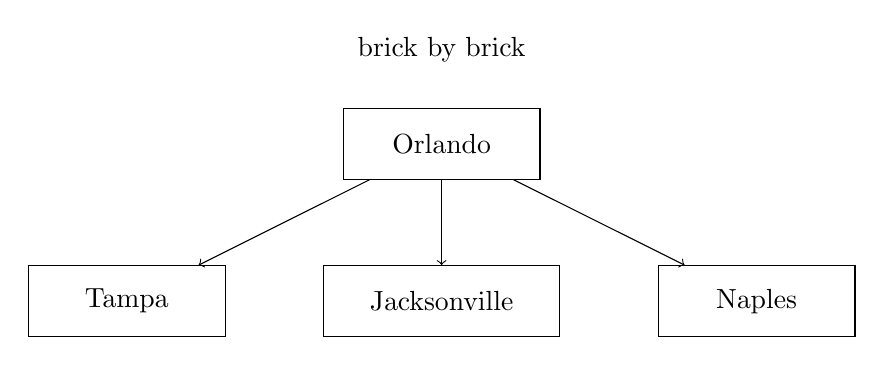
\begin{tikzpicture}[x=1cm,y=1cm]
\node[draw, rectangle, minimum width=2.5cm, minimum height=0.9cm] (o) at (0,0) {Orlando};
\node[draw, rectangle, minimum width=2.5cm, minimum height=0.9cm] (t) at (-4,-2) {Tampa};
\node[draw, rectangle, minimum width=3.0cm, minimum height=0.9cm] (j) at (0,-2) {Jacksonville};
\node[draw, rectangle, minimum width=2.5cm, minimum height=0.9cm] (n) at (4,-2) {Naples};
\draw[->] (o) -- (t);
\draw[->] (o) -- (j);
\draw[->] (o) -- (n);
\node at (0,1.2) {brick by brick};
\end{tikzpicture}
\caption{Transcript-derived schematic of adjacent-market expansion from Orlando outward.}
\label{fig:brick-scale-refined}
\end{figure}

\section{Keeping Money, Preparing for the Black Swan, and Closing the Machine}

After the expansion story, the interview swings back to scale markers. Morgan repeats the claim that the firm did about \$2 billion in fees, adds that the margins are good, and says plainly that the firm has no debt. The host then asks whether he is a billionaire, and Morgan gives an answer that is more interesting than a yes or no. He says, in effect, that exact net worth is unstable. People say they know what they are worth, but fortunes move, public estimates move, and comfort is a better description than a fixed scalar.

That is an important motivational beat. The lecture is moving from making money to keeping it. Morgan's first law in this territory is severe: it is hard to make money; it is harder to keep money. The losses, he says, come when greed takes over and one enters situations that already smell wrong. Hence the plain maxim: if it is too good to be true, it is too good to be true.

The tree-planting image then appears. The best time to plant a tree was twenty years ago; the next best time is today. This is not a financial formula, but it carries a real temporal structure. The point is to break the paralysis of retrospective regret. One does not recover the missed start by meditating on it; one starts the compounding process now.

Morgan's caution then sharpens again in a different register. He says that if he does not understand something, he does not do it, and he uses crypto as the example. This is not a universal theorem about asset classes. It is a discipline of epistemic restraint: do not let greed force capital into opaque structures merely because they are fashionable.

When the host asks where the money actually goes, the answer becomes concrete. Morgan names index funds for equities, tax-free bonds yielding roughly \(4\%\) to \(4.5\%\), U.S.\ Treasuries, and self-investment into attractions, hotels, shopping centers, and apartments. He also adds a historical claim about municipal bonds in the Great Depression. We record the financial part of the claim cautiously as
\begin{equation}
y_{\mathrm{muni}} \approx 4\%\text{ to }4.5\%, \qquad \delta_{\mathrm{muni}} < 1\%,
\end{equation}
where \(y_{\mathrm{muni}}\) denotes the bond yield and \(\delta_{\mathrm{muni}}\) the cited default rate. The second quantity is Morgan's historical assertion, not an independently verified result supplied by the lecture.

He then states the long-hold rule that governs the investment bucket: once the money goes into investments, he never touches it. In transcript-derived shorthand,
\begin{equation}
K_{t+1}^{\mathrm{invest}} = (1+r_t)K_t^{\mathrm{invest}},
\qquad
D_t^{\mathrm{invest}} = 0,
\end{equation}
where \(K_t^{\mathrm{invest}}\) is long-term investment capital, \(r_t\) its return rate, and \(D_t^{\mathrm{invest}}\) the withdrawal stream. This is not a full portfolio model. It is a compact way of preserving the lecture's insistence that permanent capital should compound instead of being repeatedly cannibalized.

The book that Morgan names as most important is \emph{The Black Swan}. His reading of it is practical rather than literary: be prepared. In the interview, preparedness immediately means savings and no debt. We may compress the doctrine as
\begin{equation}
\mathcal{P} = (\text{cash reserves},\, L=0,\, \text{readiness for shock}),
\end{equation}
with \(L\) denoting leverage. The lecture's musical-chairs metaphor then restates the same point in the language of timing:
\begin{equation}
\text{liquidity}(t^{*}) < \text{obligations}(t^{*}) \quad \Longrightarrow \quad \text{failure at shock time } t^{*}.
\end{equation}
Here again the equation is ours, not Morgan's. It merely translates his claim that when the music stops, one either has a chair or does not.

\subsection{A Worked Advertising Example}

The host now poses a useful objection. If conservative capital preservation matters so much, why spend so aggressively on advertising? Morgan's answer is one of the clearest pieces of arithmetic in the interview. He says the firm spends about \$400 million per year on advertising, while generating about \$5 billion in settlements and verdicts and about \$2 billion in fees. Using his own figures, we write
\begin{align}
A &\approx \$4 \times 10^8, &
S &\approx \$5 \times 10^9, &
F &\approx \$2 \times 10^9.
\end{align}
From these,
\begin{align}
\frac{A}{S}
&=
\frac{\$4 \times 10^8}{\$5 \times 10^9}
=
0.08,\\[4pt]
\frac{A}{F}
&=
\frac{\$4 \times 10^8}{\$2 \times 10^9}
=
0.20.
\end{align}

These ratios are genuinely helpful, but only if we keep the denominators distinct. \(S\) is client recoveries; \(F\) is firm fees. The lecture's arithmetic therefore supports two different interpretations of advertising intensity, and one must not collapse them.

Morgan's own explanation is more structural than arithmetic. There are, he says, two things in his business: catching fish and cooking fish. The first is marketing and case acquisition. The second is the legal capacity to obtain verdicts and settlements. We may write the mechanism schematically as
\begin{equation}
\text{marketing} \to \text{cases acquired} \to \text{verdict / settlement capacity} \to F.
\end{equation}

\begin{figure}
\centering
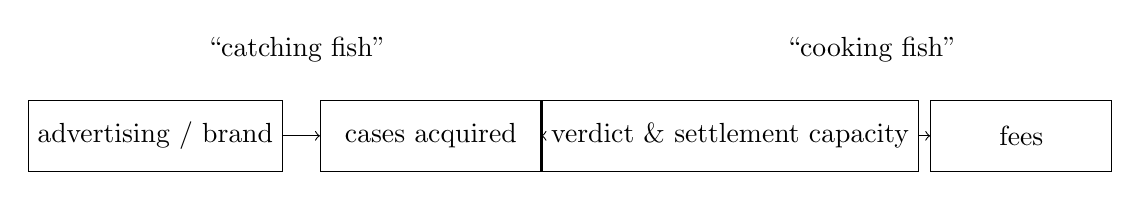
\begin{tikzpicture}[x=1cm,y=1cm]
\node[draw, rectangle, minimum width=2.9cm, minimum height=0.9cm] (m) at (-5,0) {advertising / brand};
\node[draw, rectangle, minimum width=2.8cm, minimum height=0.9cm] (c) at (-1.5,0) {cases acquired};
\node[draw, rectangle, minimum width=3.7cm, minimum height=0.9cm] (v) at (2.3,0) {verdict \& settlement capacity};
\node[draw, rectangle, minimum width=2.3cm, minimum height=0.9cm] (f) at (6,0) {fees};
\draw[->] (m) -- (c);
\draw[->] (c) -- (v);
\draw[->] (v) -- (f);
\node at (-3.2,1.1) {``catching fish''};
\node at (4.1,1.1) {``cooking fish''};
\end{tikzpicture}
\caption{Transcript-derived schematic of the two-stage revenue machine.}
\label{fig:fish-refined}
\end{figure}

This is why the interview immediately brings in real litigation strength. Morgan says the insurance industry knows who he is because the firm wins real verdicts, not make-believe ones, and he names the software system Colossus as evidence that insurers model how particular firms behave on cases. The scale marker here is
\begin{equation}
D_{\mathrm{week}} \approx 200 \text{ dockets per week}.
\end{equation}
That number tells us why advertising alone is not the engine. The engine is the coupling of front-end demand generation to back-end trial capacity.

The lecture does not stop with arithmetic. From the fish metaphor it moves into competitive posture. Morgan describes suing giant defendants, invokes David against Goliath, and says that when the other side shoots real bullets, he shoots real bombs. This is not a quantified claim, but it clarifies why the back end matters. A paper tiger may advertise; it cannot credibly threaten trial.

Branding then arrives in a way that preserves the interview's tone. One must make the creative creative; one must be willing to be memorable rather than interchangeable. But the lecture refuses to separate brand from trust. People want a winner because they want to win. The brand works only if it persuades the client that hiring this firm changes the expected quality of the fight.

The final movement widens once more, exactly as the teaser promised at the beginning. The host asks for a last guiding principle, and Morgan answers with the golden rule. He says he believes in karma, and then, in the final exchange, cites \emph{Give and Take}: takers are easy to identify and easy to guard against, but givers who lift others become trusted, and trust returns value over time. This is a fitting close. The chapter began by asking how a firm becomes a machine. It ends by saying that even a very large machine still depends on reciprocity, memory, and the long horizon of reputation.

\section{Summary}

We may now state the chapter's machine compactly. First, scale comes from delegated trust and shared upside rather than founder overextension. Second, the firm's economics depend on contingent participation in outcomes rather than the sale of hours. Third, national reach is conceived as low-friction availability, but only works when paired with real legal execution. Fourth, wealth is preserved by resisting greed, avoiding leverage, and holding permanent capital for the long run. Finally, the lecture refuses to end in arithmetic alone. It closes, as the interview closes, on trust, reciprocity, and the claim that durable commercial power is inseparable from the way one treats other people.